\documentclass{beamer}
%\usetheme{Boadilla}
\usetheme{DarkConsole}
\usepackage{courier}
\usepackage[T1]{fontenc}
\usepackage{graphicx}
\usepackage{multicol}
\usepackage{tikz}
\usepackage{hyperref}
\usetikzlibrary{calc}
\graphicspath{ {./images} }

\title {Docker}
\author {Henrique Yara}
\institute {opus-software}

\begin{document}

\begin{frame}{\titlepage}
	\begin{figure}[htpb]
		\centering
		\includegraphics[width=0.5\textwidth]{./assets/Docker_logo.png}
		\caption{Docker logo}
	\end{figure}
\end{frame}

\begin{frame}{Índice}
	\tableofcontents
\end{frame}

%\setbeamercovered{transparent}

\section{Introdução}

\begin{frame}
\frametitle{O que é docker?}
Gerenciar a infra-estrutura:
\begin{itemize}
	\item \uncover<1->{Ambientes "isolados" usando container;}
	\item \uncover<2->{Agilizar as entregas das aplicações;}
	\item \uncover<3->{Aplicações seguras;}
	\item \uncover<4->{Portabilidade;}
\end{itemize}
\end{frame}

\begin{frame}
\frametitle{O que é um container?}
\begin{itemize}
	\item Containers:
		\begin{itemize}
			\item \uncover<1->{Usa o \textit{kernel} da máquina \textit{host};}
			\item \uncover<2->{Contém:}
				\begin{itemize}
					\item \uncover<2->{\textit{Softwares};}
					\item \uncover<3->{Bibliotecas;}
				\end{itemize}
			\item \uncover<4->{Leves (Somente o necessário);}
			\item \uncover<5->{Execução quase igual à execução nativa;}
		\end{itemize}
\end{itemize}
\end{frame}

\begin{frame}
\frametitle{Características do container}
\begin{itemize}
\item \uncover<1->{Portabilidade:}
	\begin{itemize}
		\item \uncover<1->{Fácil compartilhar;}
		\item \uncover<2->{Ambiente igual para todos;}
		\item \uncover<3->{A mesma execução para todos;}
	\end{itemize}
\item \uncover<4->{Alternativa viável para as máquinas virtuais (hypervisor):}
	\begin{itemize}
		\item \uncover<4->{Melhor uso da capacidade do seu computador;}
		\item \uncover<5->{Ambientes grandes e densos;}
		\item \uncover<6->{Ambientes pequenos ou médios;}
	\end{itemize}
\end{itemize}
\end{frame}

\begin{frame}
\frametitle{Máquina virtual X Container}
\begin{multicols}{2}
\begin{itemize}
	\item Máquina Virtual
		\begin{itemize}
			\item \uncover<1->{Virtualiza a camada de aplicação e a camada do SO;}
			\item \uncover<3->{Mais pesado (Na casa dos Gigabytes);}
			\item \uncover<5->{Demoram mais para inicializar;}
			\item \uncover<7->{Executa qualquer sistema operacional em qualquer Sistema Operacional;}
		\end{itemize}
\end{itemize}
\columnbreak
\begin{itemize}
	\item Container
		\begin{itemize}
			\item \uncover<2->{Virtualiza a camada de aplicação;}
			\item \uncover<4->{Mais leve (Na casa dos megabytes);}
			\item \uncover<6->{Inicializam rapidamente;}
			\item \uncover<8->{O sistema operacional precisa ser compatível com a máquina principal ou usar uma camada de compatibilidade;}
		\end{itemize}
\end{itemize}
\end{multicols}
\end{frame}

\begin{frame}
\frametitle{Máquina virtual X Container (Imagens)}
\centering
\begin{multicols}{2}
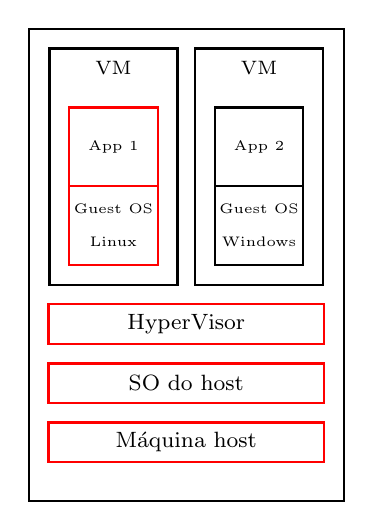
\begin{tikzpicture}
	\coordinate (A) at (0,0);
	\coordinate (B) at (0,-2.25);
	\coordinate (C) at (0,-0.75);
	\coordinate (D) at (0,-1.5);
	\coordinate (E) at (-0.925,1.25);
	\coordinate (F) at (0.925,1.25);
	\coordinate (G) at (0.925,1.5);
	\coordinate (H) at (0.925,0.5);
	\coordinate (I) at (-0.925,1.5);
	\coordinate (J) at (-0.925,0.5);
	\node at (A) [draw,thick,minimum width=4cm,minimum height=6cm] {};
	\node at (B) [draw,thick,minimum width=3.5cm,minimum height=0.5cm] {};
	\onslide<2>{\node at (B) [draw,red,thick,minimum width=3.5cm,minimum height=0.5cm] {};}
	\node at (B) {\footnotesize Máquina host};
	\node at (C) [draw,thick,minimum width=3.5cm,minimum height=0.5cm] {};
	\onslide<4>{\node at (C) [draw,red,thick,minimum width=3.5cm,minimum height=0.5cm] {};}
	\node at (C) {\footnotesize HyperVisor};
	\node at (D) [draw,thick,minimum width=3.5cm,minimum height=0.5cm] {};
	\onslide<3>{\node at (D) [draw,red,thick,minimum width=3.5cm,minimum height=0.5cm] {};}
	\node at (D) {\footnotesize SO do host};
	\node at (E) [draw,thick,minimum width=1.625cm,minimum height=3cm] {};
	\node at ($(E)+(0,1.25)$) {\scriptsize VM};
	\node at (F) [draw,thick,minimum width=1.625cm,minimum height=3cm] {};
	\node at ($(F)+(0,1.25)$) {\scriptsize VM};
	\node (rect) at (G) [draw,thick,minimum width=1.125cm,minimum height=1cm] {};
	\node at (G) {\tiny App 2};
	\node at (H) [draw,thick,minimum width=1.125cm,minimum height=1cm] {};
	\node[align=center] at (H) {\tiny Guest OS\\ \tiny Windows};
	\node at (I) [draw,thick,minimum width=1.125cm,minimum height=1cm] {};
	\node at (I) {\tiny App 1};
	\node at (J) [draw,thick,minimum width=1.125cm,minimum height=1cm] {};
	\onslide<5>{\node (rect) at (I) [red,draw,thick,minimum width=1.125cm,minimum height=1cm] {};}
	\onslide<5>{\node (rect) at (J) [red,draw,thick,minimum width=1.125cm,minimum height=1cm] {};}
	\node[align=center] at (J) {\tiny Guest OS\\ \tiny Linux};
\end{tikzpicture}
\columnbreak
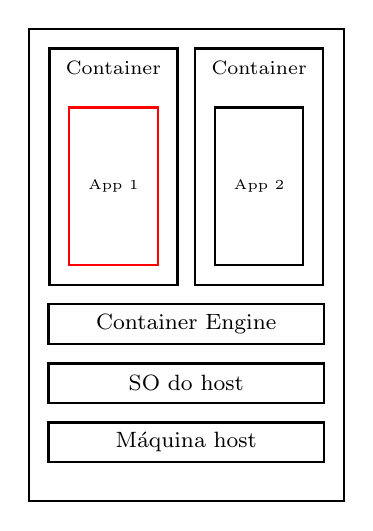
\begin{tikzpicture}
	\coordinate (A) at (0,0);
	\coordinate (B) at (0,-2.25);
	\coordinate (C) at (0,-0.75);
	\coordinate (D) at (0,-1.5);
	\coordinate (E) at (-0.925,1.25);
	\coordinate (F) at (0.925,1.25);
	\coordinate (G) at (0.925,1);
	\coordinate (H) at (-0.925,1);
	\node (rect) at (A) [draw,thick,minimum width=4cm,minimum height=6cm] {};
	\node (rect) at (B) [draw,thick,minimum width=3.5cm,minimum height=0.5cm] {};
	\node at (B) {\footnotesize Máquina host};
	\node (rect) at (C) [draw,thick,minimum width=3.5cm,minimum height=0.5cm] {};
	\node at (C) {\footnotesize Container Engine};
	\node (rect) at (D) [draw,thick,minimum width=3.5cm,minimum height=0.5cm] {};
	\node at (D) {\footnotesize SO do host};
	\node (rect) at (E) [draw,thick,minimum width=1.625cm,minimum height=3cm] {};
	\node at ($(E)+(0,1.25)$) {\scriptsize Container};
	\node (rect) at (F) [draw,thick,minimum width=1.625cm,minimum height=3cm] {};
	\node at ($(F)+(0,1.25)$) {\scriptsize Container};
	\node (rect) at (G) [draw,thick,minimum width=1.125cm,minimum height=2cm] {};
	\node at (G) {\tiny App 2};
	\node (rect) at (H) [draw,thick,minimum width=1.125cm,minimum height=2cm] {};
	\onslide<5>{\node (rect) at (H) [red,draw,thick,minimum width=1.125cm,minimum height=2cm] {};}
	\node[align=center] at (H) {\tiny App 1};
\end{tikzpicture}
\end{multicols}
\end{frame}

\begin{frame}
\frametitle{Onde os containers podem ser encontrados?}
\begin{itemize}
	\item Repositórios privados:
		\begin{itemize}
			\item Repostórios das empresas;
		\end{itemize}
	\item \uncover<2->{Repositórios públicos:}
		\begin{itemize}
			\item \uncover<2->{Docker hub;}
		\end{itemize}
\end{itemize}
\end{frame}


\section{Desenvolvimento e Execução}

\begin{frame}
\frametitle{Desenvolvimento e Execução - Objetivos}
\begin{itemize}
	\item Ambientes ``isolados``:
		\begin{itemize}
			\item \uncover<1->{Não é necessário instalar softwares dependentes na máquina principal;}
			\item \uncover<2->{Evita conflitos de versão;}
			\item \uncover<3->{Abstrair a parte da infra-estrutura aplicação;}
			\item \uncover<4->{Toda a infraestrutura pode ser facilmente executada na máquinal local;}
		\end{itemize}
\end{itemize}
\end{frame}

\section{Entrega}

\begin{frame}
	\frametitle{Entrega - Objetivos}
	\begin{itemize}
	\item Ambientes ``isolados``:
		\begin{itemize}
			\item \uncover<1->{Ambiente de testes $=$ Ambiente de produção;}
			\item \uncover<2->{Entregas de software de forma mais rápida;}
				\begin{itemize}
					\item \uncover<2->{Não é necessário instalar dependências nas máquinas ($\uparrow$ tempo);}
				\end{itemize}
		\end{itemize}
	\end{itemize}
\end{frame}

\begin{frame}
\frametitle{Entrega - CI/CD}
\begin{itemize}
	\item Docker é ótimo para \textit{continuous delivery} e \textit{continuous integration}:
		\begin{itemize}
			\item \uncover<1->{Desenvolvedores fazem mudanças no código localmente;}
			\item \uncover<2->{No ambiente de teste são executados testes manuais e automáticos;}
			\item \uncover<3->{Erros podem ser reproduzidos e arrumados usando docker;}
			\item \uncover<4->{Então a imagem vai para o ambiente de produção;}
		\end{itemize}
\end{itemize}
\end{frame}

\begin{frame}
\frametitle{Entrega - Produção e escalabilidade}
\begin{itemize}
	\item Responsive deployment and scaling
		\begin{itemize}
			\item \uncover<1->{Pode ser executado em:}
				\begin{itemize}
					\item \uncover<1->{Máquinas físicas;}
					\item \uncover<2->{Máquinas virtuais;}
					\item \uncover<3->{Data centers;}
					\item \uncover<4->{Nuvem;}
					\item \uncover<5->{Misto;}
				\end{itemize}
			\item \uncover<6->{Portabilidade $\rightarrow$ escalar os projetos ou retirar aplicações e serviços (Quase tempo real);}
		\end{itemize}
\end{itemize}
\end{frame}

\begin{frame}
\frametitle{Ciclo de vida}
\framesubtitle{Ciclo de vida}
\begin{itemize}
	\item \uncover<1->{Desenvolver: Aplicação e componentes isolados no container;}
	\item \uncover<2->{Execução: Testar e distribuir containers;}
	\item \uncover<3->{Entrega: Ambiente de produção usando container ou serviço orquestrado;}
\end{itemize}
\end{frame}

\section{Arquitetura}

\begin{frame}
\frametitle{Arquitetura do docker}
\begin{itemize}
	\item Arquitetura cliente-servidor:
		\begin{itemize}
			\item Cliente docker se comunica com o servidor do docker;
			\item \uncover<2->{Comunicação usando sockets UNIX ou pela interface de redes usando uma API REST;}
			\item \uncover<3->{O servidor é o responsável por criar imagens, rodar imagens e distribuir;}
			\item \uncover<4->{Podem rodar na mesma máquina ou em máquinas diferentes;}
		\end{itemize}
\end{itemize}
\end{frame}

\begin{frame}
\frametitle{Arquitetura do docker}
\centering
\begin{tikzpicture}
	% Coordinate A
	\coordinate (A) at (0,0);
	\node at ($(A)-(0,2.75)$) [draw,thin,minimum width=3.5cm,minimum height=5cm] {};
	\node at (A) [draw,thick,minimum width=3.5cm,minimum height=0.5cm] {};
	\node at ($(A)-(0,0.2)$)[above] { \tiny Docker client};
	\node (dbuild) at ($(A)-(0,0.9)$) [draw,thin,minimum width=3cm,minimum height=0.5cm] { \tiny Docker build};
	\node (dpull) at ($(A)-(0,2.1)$) [draw,thin,minimum width=3cm,minimum height=0.5cm]  {\tiny Docker pull};
	\node (drun) at ($(A)-(0,3.3)$) [draw,thin,minimum width=3cm,minimum height=0.5cm]  {\tiny Docker run};
	\node (detc) at ($(A)-(0,4.5)$) [draw,thin,minimum width=3cm,minimum height=0.5cm]  {\tiny \dots};

	% Coordinate B
	\coordinate (B) at ($(1,0)+(3,0)+(A)$);
	\node at ($(B)-(0,2.75)$) [draw,thin,minimum width=3.5cm,minimum height=5cm] {};
	\node at (B) [draw,thick,minimum width=3.5cm,minimum height=0.5cm] {};
	\node at ($(B)-(0,0.2)$)[above] {\tiny Docker host};
	\node (ddaemon) at ($(B)-(0,0.9)$) [draw,thin,minimum width=3cm,minimum height=0.5cm] { \tiny Docker daemon};
	\node (rect) at ($(B)-(0.8,2.1)$) [draw,thick,minimum width=1.4cm,minimum height=0.5cm]  {\tiny Container};
	\node (rect) at ($(B)-(-0.8,2.1)$) [draw,thick,minimum width=1.4cm,minimum height=0.5cm]  {\tiny Image};
	\node (rect) at ($(B)-(0.8,3.55)$) [draw,thin,minimum width=1.4cm,minimum height=2.4cm]  {};
	\node[inner sep=0pt] (docker) at ($(B)-(0.8,2.8)$)
    {\includegraphics[width=.05\textwidth]{./assets/Docker_logo.png}};
	\node[inner sep=0pt] at ($(B)-(0.8,3.6)$)
    {\includegraphics[width=.05\textwidth]{./assets/Docker_logo.png}};
	\node[inner sep=0pt] at ($(B)-(0.8,4.4)$)
    {\includegraphics[width=.05\textwidth]{./assets/Docker_logo.png}};
	\node (rect) at ($(B)-(-0.8,3.55)$) [draw,thin,minimum width=1.4cm,minimum height=2.4cm]  {};
	\node[inner sep=0pt] (ubuntu2) at ($(B)-(-0.8,2.8)$)
    {\includegraphics[width=.05\textwidth]{./assets/Ubuntu.png}};
	\node[inner sep=0pt] at ($(B)-(-0.8,3.6)$)
    {\includegraphics[width=.05\textwidth]{./assets/Fedora.png}};
	\node[inner sep=0pt] (amazon2) at ($(B)-(-0.8,4.4)$)
    {\includegraphics[width=.05\textwidth]{./assets/Amazon.png}};

	% Coordinate C
	\coordinate (C) at ($(1,0)+(3,0)+(B)$);
	\node at ($(C)-(0,2.75)$) [draw,thin,minimum width=3.5cm,minimum height=5cm] {};
	\node at (C) [draw,thick,minimum width=3.5cm,minimum height=0.5cm] {};
	\node at ($(C)-(0,0.2)$)[above] {\tiny Registry};
	\node[inner sep=0pt] at ($(C)-(0.8,1.25)$) {\includegraphics[width=.10\textwidth]{./assets/Ubuntu.png}};
	\node[inner sep=0pt] at ($(C)-(-0.8,2.75)$) {\includegraphics[width=.10\textwidth]{./assets/Fedora.png}};
	\node[inner sep=0pt] (amazon) at ($(C)-(0.8,4.25)$) {\includegraphics[width=.10\textwidth]{./assets/Amazon.png}};
	

	% Lines
	\draw[-,thin,dotted] (dbuild.east) -- (ddaemon.west);
	\onslide<2>{\draw[-,red,thick,dotted] (dbuild.east) -- (ddaemon.west);}
	\draw[-,thin,dotted] (ddaemon.east) to[out=-20,in=-30] (ubuntu2.east);
	\onslide<3>{\draw[-,red,thick,dotted] (ddaemon.east) to[out=-20,in=-30] (ubuntu2.east);}

	\draw[-,thin,dashed] (dpull.east) -- (ddaemon.west);
	\onslide<4>{\draw[-,red,thick,dashed] (dpull.east) -- (ddaemon.west);}
	\draw[-,thin,dashed] (ddaemon.east) -- (amazon.west);
	\onslide<5>{\draw[-,red,thick,dashed] (ddaemon.east) -- (amazon.west);}
	\draw[-,thin,dashed] (amazon.west) -- (amazon2.east);
	\onslide<6>{\draw[-,red,thick,dashed] (amazon.west) -- (amazon2.east);}

	\draw[-,thin] (drun.east) -- (ddaemon.west);
	\onslide<7>{\draw[-,red,thick] (drun.east) -- (ddaemon.west);}
	\draw[-,thin] (detc.east) -- (ddaemon.west);

	\draw[->,thin] (ddaemon.south) -- (ubuntu2.west);
	\onslide<8>{\draw[->,red,thick] (ddaemon.south) -- (ubuntu2.west);}
	\draw[->,thin] (ubuntu2.west) -- (docker.east);
	\onslide<9>{\draw[->,red,thick] (ubuntu2.west) -- (docker.east);}
\end{tikzpicture}
\end{frame}

\section{Docker Objects}

\begin{frame}
\frametitle{Docker Objects - Imagem}
\begin{itemize}
	\item É um \textbf{template}. Portanto, só é permitido ler;
	\item \uncover<2->{Contém instruções para criar um container de \textit{Docker};}
	\item \uncover<3->{Uma \textbf{Imagem} é composta por camadas;}
	\item \uncover<4->{Camada inicial $\rightarrow$ Imagem pequena de Linux;}
	\item \uncover<5->{Imagens existentes $\rightarrow$ Customizadas para gerar novas imagens;}
\end{itemize}
\end{frame}

\begin{frame}[t]
\frametitle{Docker Objects - Imagem personalizada}
\begin{itemize}
	\item Para construir a uma imagem customizada, é preciso construir um \textit{Dockerfile}.
	\item \uncover<2->{\textit{Dockerfile}:}
		\begin{itemize}
			\item \uncover<2->{Arquivo com instruções para construir e executar uma imagem de um container;}
			\item \uncover<3->{Cada instrução no arquivo Dockerfile adiciona uma camada nova na imagem;}
		\end{itemize}
\begin{center}

\begin{multicols}{2}
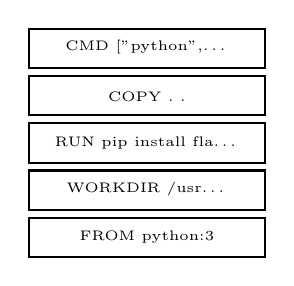
\begin{tikzpicture}
	\coordinate (A) at (0,0);
	\coordinate (B) at (0,0.6);
	\coordinate (C) at (0,1.2);
	\coordinate (D) at (0,1.8);
	\coordinate (E) at (0,2.4);
	\uncover<4->{\node (rect) at (A) [draw,thick,minimum width=3cm,minimum height=0.5cm] {};}
	\uncover<4->{\node at ($(A)-(0,0.2)$)[above] {\tiny FROM python:3};}
	\uncover<5->{\node (rect) at (B) [draw,thick,minimum width=3cm,minimum height=0.5cm] {};}
	\uncover<5->{\node at ($(B)-(0,0.2)$)[above] {\tiny WORKDIR /usr\dots};}
	\uncover<6->{\node (rect) at (C) [draw,thick,minimum width=3cm,minimum height=0.5cm] {};}
	\uncover<6->{\node at ($(C)-(0,0.2)$)[above] {\tiny RUN pip install fla\dots};}
	\uncover<7->{\node (rect) at (D) [draw,thick,minimum width=3cm,minimum height=0.5cm] {};}
	\uncover<7->{\node at ($(D)-(0,0.2)$)[above] {\tiny COPY . .};}
	\uncover<8->{\node (rect) at (E) [draw,thick,minimum width=3cm,minimum height=0.5cm] {};}
	\uncover<8->{\node at ($(E)-(0,0.2)$)[above] {\tiny CMD ["python",\dots};}
\end{tikzpicture}
\columnbreak
\begin{tikzpicture}
	\uncover<9->{\node (rect) at (A) [red,draw,thick,minimum width=3cm,minimum height=0.5cm] {};}
	\uncover<9->{\node at ($(A)-(0,0.2)$)[above] {\tiny FROM python:3};}
	\uncover<10->{\node (rect) at (B) [red,draw,thick,minimum width=3cm,minimum height=0.5cm] {};}
	\uncover<10->{\node at ($(B)-(0,0.2)$)[above] {\tiny WORKDIR /usr\dots};}
	\uncover<11->{\node (rect) at (C) [draw,thick,minimum width=3cm,minimum height=0.5cm] {};}
	\uncover<11->{\node at ($(C)-(0,0.2)$)[above] {\tiny RUN pip install  uvi\dots};}
	\uncover<12->{\node (rect) at (D) [draw,thick,minimum width=3cm,minimum height=0.5cm] {};}
	\uncover<12->{\node at ($(D)-(0,0.2)$)[above] {\tiny COPY . .};}
	\uncover<13->{\node (rect) at (E) [draw,thick,minimum width=3cm,minimum height=0.5cm] {};}
	\uncover<13->{\node at ($(E)-(0,0.2)$)[above] {\tiny  ENTRYPOINT u\dots};}
\end{tikzpicture}
\end{multicols}

\end{center}
\end{itemize}
\end{frame}

\begin{frame}
\frametitle{Docker Objects - Imagem}
\framesubtitle{Imagem}
\begin{itemize}
	\item Novas customizações $\rightarrow$ Novas camadas na Imagem;
	\item \uncover<2->{Na construção de uma imagem, apenas as camadas que sofreram mudanças vão ser reconstruídas;}
	\item \uncover<3->{Imagens leves, pequenas e rápidas (Comparadas com outras tecnologias);}
\end{itemize}
\end{frame}

\begin{frame}[t]
\frametitle{Docker Objects - Containers}
\begin{itemize}
	\item Instância de uma imagem;
		\begin{itemize}
			\item Configurações definidas na inicialização e na imagem;
			\item \uncover<2->{Mudanças no container não são armazenadas;}
		\end{itemize}
	\item \uncover<3->{Com a API do docker é possível:}
		\begin{itemize}
			\item \uncover<3->{Criar um container;}
			\item \uncover<4->{Executar um container;}
			\item \uncover<5->{Parar um container;}
			\item \uncover<6->{Mover um container;}
			\item \uncover<7->{Deletar um container;}
		\end{itemize}
	\item \uncover<8->{Gerenciar:}
		\begin{itemize}
			\item \uncover<8->{Redes;}
			\item \uncover<9->{Armazenamento;}
			\item \uncover<10->{Imagem;}
		\end{itemize}
\end{itemize}
\end{frame}

\begin{frame}[t]
\frametitle{Docker Objects - Tecnologias}
\begin{itemize}
	\item Linguagem \textbf{Go};
	\item \uncover<2->{Muitas funcionalidades do kernel do linux:}
		\begin{itemize}
			\item \uncover<2->{namespaces: Garante que cada um dos containers tenha a capacidade de se isolar em níveis:}
			\begin{itemize}
				\item \uncover<3->{PID: Ter seus próprios PIDs, mas a máquina host pode ver os PIDs do container;}
				\item \uncover<3->{NET: Ter suas próprias interfaces de redes e portas. Responsável pela comunicação de containers;}
				\item \uncover<3->{MNT: Garante que um sistema de arquivos montado não consiga acessar outro sistema de arquivos montado por outro mnt;}
				\item \uncover<3->{IPC: Ter um SystemV IPC isolado, além de uma fila de mensagems POSIX própria;}
				\item \uncover<3->{UTS: Isolamento do hostname, nome do domínio, versão do SO, etc...;}
			\end{itemize}
			\item \uncover<4->{cgroups: Garantir o controle do consumo de processo;}
			\item \uncover<5->{Linux Security Modules: Permissões do que eu sou permitido fazer;}
		\end{itemize}
\end{itemize}
\end{frame}

\begin{frame}[t]
\frametitle{Docker Objects - Container Runtimes}
\begin{itemize}
	\item As ferramentas \textbf{Container Runtimes} são ferramentas que facilitam a criação de containers de forma isolada e segura.
	\item Open container Initiative runtimes:
		\begin{itemize}
			\item Native Runtimes:
			\begin{itemize}
				\item runC: escrito em go e mantido pelo projeto moby do docker;
				\item Railcar: escrito em rust, mas foi abandonado;
				\item Crun: escrito em c, performatico e leve;
			\end{itemize}
		\end{itemize}
	\item Container Runtime Interface
		\begin{itemize}
			\item containerd: um runtime de alto nível desenvolvido no projeto moby do docker, por padrão usa o runC por baixo dos panos;
			\item cri-o: implementação liderada pela Redhat, feita especificamente para o kubernetes;
		\end{itemize}
\end{itemize}
\end{frame}

\begin{frame}
\frametitle{Docker Objects - Resumo}
\begin{itemize}
	\item Daemon (dockerd): espera por chamads API do docker, e gerencia objetos como imagens, containers, redes e volumes;
	\item \uncover<2->{Cliente (docker): interage com o dockerd;}
		\begin{itemize}
			\item \uncover<2->{Comandos como: docker run, o cliente envia comandos para o dockerd;}
			\item \uncover<3->{O cliente docker pode se comunicar com mais de um daemon;}
		\end{itemize}
	\item \uncover<4->{Docker desktop: é uma aplicação fácil de ser instalada nos ambientes Mac, Windows ou Linux.}
		\begin{itemize}
			\item \uncover<5->{O docker desktop contém o daemon (dockerd), o docker client (docker), docker compose, docker content trust, kubernetes e credential helper;}
		\end{itemize}
\end{itemize}
\end{frame}

\begin{frame}
\frametitle{Docker Objects - Resumo}
\begin{itemize}
	\item Docker registries: Guarda as imagens de docker;
		\begin{itemize}
			\item Docker Hub: é um registro público, por padrão o docker procura por imagens no Docker Hub;
			\item \uncover<2->{É possível ter até seu registro próprio;}
			\item \uncover<3->{Os comandos docker pull, docker run e docker push procuram ou enviam as imagens para o registro configurado na máquina que estão rodando;}
		\end{itemize}
	\item \uncover<4->{Docker objects: Imagens, conteiners, redes, volumes, plugins, etc...}
\end{itemize}
\end{frame}

\section{Volumes}

\begin{frame}
	\frametitle{Volumes}
	\begin{itemize}
		\item \uncover<1->{Os volumes são formas de armazenar informações persistentes para uso futuro.}
		\item \uncover<2->{Tipos de volumes:}
			\begin{itemize}
				\item \uncover<2->{Volumes: Os volumes são gerenciados pelo próprio \textbf{docker}.}
				\item \uncover<3->{Bint mounts: É possível montar diretórios dentro do container, dessa forma o container pode acessar arquivos que existem dentro da máquina host.}
				\item \uncover<4->{Tmpfs: O \textbf{tmpfs} é uma forma de evitar armazenar dados permanenteente, e melhora a performace do container evitando escrever na camada de escrita do container}
			\end{itemize}
	\end{itemize}
\end{frame}

\section{Redes}

\begin{frame}
	\frametitle{Redes - Bridge}
	\begin{itemize}
		\item \uncover<1->{Usar a interface de rede \textbf{docker0};}
			\begin{itemize}
				\item \uncover<1->{Cada container vai ter um veth (Virtual ethernet interface);}
				\item \uncover<2->{Cada veth vai estar conectado com o docker0;}
			\end{itemize}
		\item \uncover<3->{Todos os containers na rede vão conseguir se comunicar (Ruim);}
		%\item \uncover<4->{Usa o /etc/resolv.conf da máquina local dentro do docker;}
	\end{itemize}
\end{frame}

\begin{frame}
	\frametitle{Redes - User-Defined Bridge}
	\begin{itemize}
		\item \uncover<1->{Igual ao Bridge}
		\item \uncover<2->{Mais controle das conexões entre os containers}
		\item \uncover<3->{Isolados dos containers dentro do bridge padrão}
	\end{itemize}
\end{frame}

\begin{frame}
	\frametitle{Redes - Host}
	\begin{itemize}
		\item \uncover<1->{Compartilha o ip e as portas com a máquina host}
		\item \uncover<2->{É como se fosse uma aplicação rodando no computador}
		\item \uncover<3->{Acaba não ficando isolado}
	\end{itemize}
\end{frame}

\begin{frame}
	\frametitle{Redes - macVLAN}
	\begin{itemize}
		%\item docker network create -d macvlan --subnet 10.7.1.0/24 --gateway 192.168.0.1 -o parent=enp0s3 macVLANname
		%\item docker run -itd --rm --network lan --ip 192.168.0.24 --name teste
		\item \uncover<1->{Feito para aplicações antigas que precisam conectar diretamente na internet física}
			\begin{itemize}
				\item \uncover<1->{Conseguem um enderaço MAC próprio;}
				\item \uncover<2->{Tem seus próprios IPs;}
			\end{itemize}
		\item \uncover<3->{Desvantagens:}
			\begin{itemize}
				\item \uncover<3->{Existe só um endereço MAC;}
					\begin{itemize}
						\item \uncover<3->{Precisa do modo Prosmiscuous (Um endereço físico pode ter múltiplos endereços MAC)}
					\end{itemize}
				\item \uncover<4->{Vão existir o DHCP do roteador e o DHCP do docker;}
			\end{itemize}
	\end{itemize}
\end{frame}

%\begin{frame}
%	\frametitle{Redes - IPVLAN (L2)}
%	\begin{itemize}
%		\item A interface de rede da máquina é compartilhada;
%		\item Allow the host to share its interface network
%		\item docker network create -d ipvlan --subnet 192.168.20.0/24 --gateway 192.168.0.1 -o parent=enp0s3 ipVLANname
%		\item like switching
%	\end{itemize}
%\end{frame}
%
%\begin{frame}
%	\frametitle{Redes - IPVLAN (L3)}
%	\begin{itemize}
%		\item docker network create -d ipvlan --subnet 192.168.20.0/24 -o parent=enp0s3 -o ipvlan\_mode=l3 --subnet 192.168.95.0/24 ipVLANname
%		\item you dont need to specify the gateway, as it will be the host
%		\item The host becomes like a router
%		\item Layer 3
%		\item They connect to the host like he is a router
%		\item (no broadcast and no arp)
%		\item Like a UTM?
%	\end{itemize}
%\end{frame}

\section{Pratico}

\begin{frame}[t]
	\frametitle{Pratico - Docker client}
	\framesubtitle{Lista de comandos}
\begin{multicols}{2}
	\begin{itemize}
		\item docker system info
		\item docker ps [-a]
		\item docker container;
			\begin{itemize}
				\item ls;
				\item \{un,\}pause;
				\item stop;
				\item start;
				\item restart;
				\item create;
				\item run;
			\end{itemize}
		\item docker \{image,volume,network\};
		\item docker build;
	\end{itemize}
	\columnbreak
	\begin{itemize}
		\item docker history;
		\item docker inspect;
		\item docker logs;
		\item docker ports;
		\item docker stats;
		\item docker top;
	\end{itemize}
\end{multicols}
\end{frame}

\begin{frame}
	\frametitle{Pratico - Docker client}
	\framesubtitle{Lista de comandos}
%\begin{multicols}{2}
	\begin{itemize}
		\item docker commit;
		\item docker login;
		\item docker pull;
		\item docker push;
		\item docker search;
	\end{itemize}
	%\columnbreak
	%\begin{itemize}
	%	\item docker daemon:
	%		\begin{itemize}
	%			\item --insecure registry: Permite comunicação com registry inseguros Sem certificados TLS
	%			\item --bridge: Conecta os containers com uma especifica bridge
	%			\item --bip:  Especifica um IP para a bridge
	%			\item --debug: Habilita o modo debug
	%			\item --default gateway: Configura a rota padrão
	%			\item --default ulimit: Configura o ulimit para os containers
	%			\item --dns: Indica os DNS servers que os containers utilizarão
	%			\item --fixed cidr: Fixa um range de IP para utilização do Docker
	%			\item --ip forward: Habilita o net.ipv4.ip\_forward
	%			\item --ip masq: Habilita o mascaramento de IP
	%			\item --pidfile: Configura o caminho do PID file do Docker
	%			\item --selinux enabled: Habilita o SELinux
	%			\item --storage-opt: Configura outras opções de storage
	%		\end{itemize}
	%\end{itemize}
%\end{multicols}
\end{frame}

\begin{frame}
	\frametitle{Pratico - Dockerfile}
	\framesubtitle{Dockerfile}
	\begin{itemize}
		\item \textbf{FROM}: Indica qual imagem vai ser utilizada para ser a base do container;
		\item \textbf{MAINTAINER}: Autor da imagem;
		\item \textbf{LABEL}: Adiciona metadados (Versão, descrição e fabricante);
		\item \textbf{ADD}: Copia arquivos para dentro do container (Pode descomprimir alguns arquivos e pegar arquivos de URL);
		\item \textbf{COPY}: Copia arquivos e diretórios para dentro do container;
		\item \textbf{CMD}: Executar um comando no início da execução do container. Mas pode definir argumentos padrão para o \textbf{ENTRYPOINT};
	\end{itemize}
\end{frame}

\begin{frame}[t]
	\frametitle{Pratico - Dockerfile}
	\framesubtitle{Dockerfile}
	\begin{itemize}
		\item \textbf{ENTRYPOINT}: Assim como o \textbf{CMD} executa um comando no início da execução do container, mas é mais difícil sobrescrever. E pode receber argumentos do \textbf{CMD};
		\item \textbf{ENV}: Coloca variáveis de ambiente no container;
		\item \textbf{EXPOSE}: Abre uma porta para a \textbf{Rede interna};
		\item \textbf{RUN}: Executa um comando durante a criação da imagem;
		\item \textbf{USER}: Define qual usuário vai ser utilizado para executar os próximos comandos;
		\item \textbf{WORKDIR}: Define o diretório raiz;
		\item \textbf{VOLUME}: Permite a criação de um ponto de montagem no container;
	\end{itemize}
\end{frame}

\section{Segurança}

%\begin{frame}
%	\frametitle{Segurança - Thread Modeling - pt 1}
%	\begin{itemize}
%		\item Quais são os possíveis vetores de ataque?
%			\begin{itemize}
%				\item \uncover<1->{Container Escape (System);}
%					\begin{itemize}
%						\item \uncover<1->{O atacante conseguiu abrir uma shell no container do sistema;}
%						\item \uncover<2->{Ele pode ter acesso de um usuário comum ou escalar privilégios;}
%					\end{itemize}
%				\item \uncover<3->{Other Containers via Network:}
%					\begin{itemize}
%						\item \uncover<3->{Está tentando atacar outro container pela rede;}
%					\end{itemize}
%				\item \uncover<4->{Attacking the Orchestration Tool via Network:}
%					\begin{itemize}
%						\item \uncover<4->{Atacar a ferrameta de orquestração;}
%					\end{itemize}
%			\end{itemize}
%	\end{itemize}
%\end{frame}

%\begin{frame}
%	\frametitle{Segurança - Thread Modeling - pt 2}
%	\begin{itemize}
%		\item Quais são os possíveis vetores de ataque?
%			\begin{itemize}
%				\item \uncover<1->{Resource Starvation:}
%					\begin{itemize}
%						\item \uncover<1->{Usar muita CPU, RAM, internet ou armazenamento;}
%						\item \uncover<2->{Acaba afetando outros containers;}
%					\end{itemize}
%				\item \uncover<3->{Host Compromise:}
%					\begin{itemize}
%						\item \uncover<3->{Atacou diretamente o host;}
%					\end{itemize}
%				\item \uncover<4->{Integrity of Images:}
%					\begin{itemize}
%						\item \uncover<4->{Mudou a imagem em algum momento antes do deploy;}
%					\end{itemize}
%			\end{itemize}
%	\end{itemize}
%\end{frame}

\begin{frame}
	\frametitle{OWASP Docker Top 10}
	\begin{itemize}
		\item D01 - Secure User Mapping;
		\item D02 - Patch Management Strategy;
		\item D03 - Network Segmentation and Firewalling;
		\item D04 - Secure Defaults and Hardening;
		\item D05 - Maintain Security Contexts;
		\item D06 - Protect Secrets;
		\item D07 - Resource Protection;
		\item D08 - Container Image Integrity and Origin;
		\item D09 - Follow Immutable Paradigm;
		\item D10 - Logging;
	\end{itemize}
\end{frame}

\begin{frame}[t]
	\frametitle{Segurança - Ferramentas}
	\begin{itemize}
		\item Docker scan: Segurança de Imagens (Snyk)
		\item \href{https://github.com/docker/docker-bench-security}{Docker bench security}
		\item \href{https://www.cisecurity.org/benchmark/docker}{Guideline para usar docker (CIS)}
		\item InSpec (Segurança e Compliance)
		\item Lynis
		\item \href{https://github.com/OWASP/Docker-Security}{OWASP Docker-security}
		\item \href{https://github.com/kost/dockscan}{Dockscan}
		\item \href{https://www.slideshare.net/jlkinsel/a-fun-comparison-of-docker-vulnerability-scanners/}{Comparações de scanners de vulnerabilidade de containers}
		\item \href{https://sysdig.com/blog/20-docker-security-tools/}{20 de scanners de vulnerabilidade de containers}
		\item \href{https://thenewstack.io/draft-vulnerability-scanners/}{Lista de scanners de vulnerabilidade de container}
		\item SELinux (Security Enchantment Linux): Administrar permissões no Linux
			\begin{itemize}
				\item O Linux usa o DAC (Discretionary Access Control);
				\item O \textit{SELinux} permite o MAC (Mandatory Access Control);
				\item Adiciona categorias/rótulos/perfis em todos os objetos contidos no sistema de arquivos;
			\end{itemize}
	\end{itemize}
\end{frame}

%\begin{frame}[t]
%	\frametitle{Videos}
%	\begin{itemize}
%		\item How I Learned Docker Security the Hard Way (So You Don’t Have To): \url{https://www.youtube.com/watch?v=C343TPOpTzU}
%		\item Learn which Container Security checks you should implement into your Software Development Life Cycle: \url{https://www.youtube.com/watch?v=rcrmTHOIz24}
%	\end{itemize}
%\end{frame}

\section{Maquina host}

\begin{frame}
	\frametitle{Segurança - Máquina host}
	\begin{itemize}
		\item \uncover<1->{Docker-bench-security: Security auditing and benchmarktool for Docker;}
		\item \uncover<2->{The Linux Auditing Framework: Linux Auditing Framework}
		\item \uncover<3->{InSpec: Automated security and compliance Framework}
		\item \uncover<4->{Lynis: Security auditing tool for systems based on UNIX like Linux, macOS, BSD and others. \textbf{in-depht security scan} and runs on systems itself. The primary goal is to test security defenses and provide tips for further system hardening}
	\end{itemize}

\end{frame}

\begin{frame}
	\frametitle{Docker Bench Security}
	\begin{itemize}
		\item \textit{docker-bench-security} vai analisar todo o sistema e dar uma pontuação total para o seu sistema.
		\item O \textit{docker-bench-security} pode ser usado com a flag \textit{-c} e o argumento \textit{host\_configuration};
			\begin{itemize}
				\item Dessa forma vai ser rodado testes de segurança na máquina local;
			\end{itemize}
	\end{itemize}
\end{frame}

\begin{frame}
	\frametitle{The Linux Audit Framework}
	\begin{itemize}
		\item \textit{auditctl}: Vai fazer logs de alguns programas que estão rodando na máquina host.
			\begin{itemize}
				\item \textit{/run/containerd}
				\item \textit{/var/lib/docker}
				\item \textit{/etc/docker}
				\item \textit{/lib/systemd/system/docker.service}
				\item \textit{/lib/systemd/system/docker.socket}
				\item \textit{/etc/default/docker}
				\item \textit{/usr/bin/docker-containerd}
				\item \textit{/usr/bin/docker-runc}
				\item \textit{/usr/bin/containerd}
				\item \textit{/usr/bin/containerd-shim}
				\item \textit{/usr/bin/containerd-shim-runc-v1}
				\item \textit{/usr/bin/containerd-shim-runc-v2}
			\end{itemize}
	\end{itemize}
\end{frame}

\begin{frame}
	\frametitle{The Linux Audit Framework}
	\begin{itemize}
		\item \uncover<1->{As regras precisam ser adicionadas dentro do arquivo \textit{audit.rules};}
			\begin{itemize}
				\item \uncover<1->{O arquivo das regras fica armazenado no \textit{/etc/audit/rules.d/audit.rules};}
			\end{itemize}
		\item \uncover<2->{O comando \textit{aureport} vai ser usado para verificar os logs;}
	\end{itemize}
\end{frame}

\begin{frame}[t]
	\frametitle{Logins por SSH}
	\begin{itemize}
		\item Arquivo \textit{/etc/ssh/sshd\_config}
			\begin{itemize}
				\item Port: Mudar a porta do SSH (Atacante é obrigado a escanear todas as portas);
				\item \uncover<2->{LogLevel: Mudar para VERBOSE;}
				\item \uncover<3->{LoginGraceTime: Diminuir o tempo limite (O server desconecta o usuário se ele não conseguir fazer o login);}
				\item \uncover<4->{PermitRootLogin: Não permitir;}
				\item \uncover<5->{MaxAuthTries: Colocar um limite nas tentativas de autenticação;}
				\item \uncover<6->{MaxSessions: Número máximo de sessões concorrentes;}
				\item \uncover<7->{PasswordAuthentication: Desabilitar login por senha;}
				\item \uncover<8->{PublicKeyAuthentication: Habilitar (Por padrão já aceita);}
			\end{itemize}
	\end{itemize}
\end{frame}

\begin{frame}[t]
	\frametitle{Referencias}
	\begin{itemize}
		\item \href{https://www.youtube.com/watch?v=egqSNqNISz0}{Securing Docker Host}
	\end{itemize}
\end{frame}

\section{Docker Daemon}

\begin{frame}
	\frametitle{Segurança - Docker Daemon}
	\begin{itemize}
		\item \uncover<1->{Controlar acesso do grupo `docker`;}
		\item \uncover<2->{Criptografia TLS;}
		\item \uncover<3->{Implementar Namespaces do usuario;}
		\item \uncover<4->{Desabilitar comunicação entre containers na rede default;}
	\end{itemize}
\end{frame}

\begin{frame}
	\frametitle{Criptografia TLS}
	\begin{itemize}
		\item \uncover<1->{A criptografia TLS vai ficar entre o cliente do docker e o docker host}
		\item \uncover<2->{Arrumar o arquivo \textbf{/etc/docker/daemon.json:}}
		\item \uncover<3->{Arrumar o arquivo \textbf{/etc/systemd/system/docker.service.d/override.conf:}}
			\begin{itemize}
				\item \uncover<4->{--tlsverify}
				\item \uncover<4->{--tlscert=server-cert.pem}
				\item \uncover<4->{--tlscacert=ca.pem}
				\item \uncover<4->{--tlskey=server-key.pem}
			\end{itemize}
	\end{itemize}
\end{frame}

\begin{frame}
	\frametitle{Criptografia TLS}
	\begin{itemize}
		\item \uncover<1->{Arrumar variáveis de ambiente no cliente:}
			\begin{itemize}
				\item \uncover<1->{DOCKER\_TLS\_VERIFY=1;}
				\item \uncover<1->{DOCKER\_CERT\_PATH='path';}
			\end{itemize}
		\item \uncover<2->{Para recarregar:}
			\begin{itemize}
				\item \uncover<2->{systemctl daemon-reload;}
				\item \uncover<2->{systemctl restart docker;}
			\end{itemize}
		\item \uncover<3->{\href{https://github.com/AlexisAhmed/DockerSecurityEssentials/blob/main/Docker-TLS-Authentication/secure-docker-daemon.sh}{Script for TLS-Authentication}}
		\item \uncover<4->{Evitar ataque \textit{Man-in-the-middle}}
	\end{itemize}
\end{frame}

\begin{frame}[t]
	\frametitle{User Namespaces}
	\begin{itemize}
		\item \uncover<1->{Criar um usuário e grupo nos arquivos /etc/subuid e /etc/subgid;}
		\item \uncover<2->{Ou usar o usuário padrão \textbf{dockremap};}
		\item \uncover<4->{Diminuir os danos causados em caso de \textit{container breakout};}
		\item \uncover<5->{Arrumar o arquivo \textbf{/etc/docker/daemon.json:}}
		\item \uncover<5->{Arrumar o arquivo \textbf{/etc/systemd/system/docker.service.d/override.conf:}}
			\begin{itemize}
				\item userns-remap="default"
			\end{itemize}
	\end{itemize}
\end{frame}

\begin{frame}[t]
	\frametitle{Comunicação entre containers}
	\begin{itemize}
		\item \uncover<5->{Arrumar o arquivo \textbf{/etc/docker/daemon.json:}}
		\item \uncover<5->{Arrumar o arquivo \textbf{/etc/systemd/system/docker.service.d/override.conf:}}
			\begin{itemize}
				\item icc="false"
			\end{itemize}
		\item \uncover<2->{Containers dentro da rede default não vão conseguir se comunicar;}
	\end{itemize}
\end{frame}

\section{Links}

\begin{frame}[t]
	\frametitle{Links}
	\begin{itemize}
		\item Setup docker registry with TLS SSL: \url{https://www.thegeekstuff.com/2017/01/secure-docker-registry/}
		\item Generate SSL Key: \url{https://www.thegeekstuff.com/2009/07/linux-apache-mod-ssl-generate-key-csr-crt-file/}
		\item Docker Registry \url{https://github.com/marcelogomesrp/curso_docker/tree/main/15_registry}
		\item How to create your own docker registry: \url{https://gabrieltanner.org/blog/docker-registry/}
		\item Docker docs: \url{https://docs.docker.com/registry/configuration/}
		\item Docker native basich auth:\url{https://docs.docker.com/registry/deploying/\#native-basic-auth}
	\end{itemize}
\end{frame}

\begin{frame}[t]
	\frametitle{Links}
	\begin{itemize}
		\item ip addr;
		\item ps ef;
		\item ss tl;
		\item iptable;
		\item SysV;
		\item SystemD;
		\item Passar parametros:
			\begin{itemize}
				\item debian like
					\begin{itemize}
						\item vim /etc/default/docker
					\end{itemize}
				\item redhatlike
					\begin{itemize}
						\item vim /etc/sysconfig/docker
					\end{itemize}
			\end{itemize}
	\end{itemize}
\end{frame}


%curl -k -u usuario:senha https://manga.server:443/v2/_catalog
%Da até para usar aplicações CLI como se fossem locais
%Usar o docker para compilar aplicações
%Testar ferramentas (Banco de dados)
%Compartilhar aplicações
%awesome-selfhosted

\end{document}
